\documentclass{article}
\usepackage{indentfirst,amsmath, amsthm, amssymb, bm, caption, CJK, graphicx, hyperref, mathrsfs, color}

\begin{document}

    
    
    The track of the Flip Flap Railway is a perfect circle. The radius of it is $R$.

    The net force is $\frac{mv^2}{r}$, where $r$ is the radius of curvature, which is the reciprocal of curvature.
    
    For 
    $
    \varphi(t) = 
    \begin{pmatrix}
    R\cos t \\
    R\sin t
    \end{pmatrix}
    $,
    we have

    $$
    \varphi'(t) = 
    \begin{pmatrix}
    -R\sin t \\
    R\cos t
    \end{pmatrix},\ 
    T\circ\varphi(t) = 
    \begin{pmatrix}
    -\sin t \\
    \cos t
    \end{pmatrix},\ 
    (T\circ\varphi)(t) = 
    \begin{pmatrix}
    -\cos t \\
    -\sin t
    \end{pmatrix}
    $$

    By substituting the quantities, we obtain 

    $$
    \kappa=\frac{||(T\circ\varphi)'(t)||}{||\varphi'(t)||}=\frac{1}{R},
    $$

    which indicates that the radius of the curvature is a constant $R$.

    Thus, when the Flip Flap Railway reaches the lowest position, the normal force reaches max, which is:

    \begin{equation}
    N=\frac{mv_{\mathrm{bottom}}^2}{R}+mg.
    \end{equation}

    Since it's weightless at the top, we have

    \begin{equation}
    \frac{mv_{\mathrm{top}}^2}{R}=mg.
    \end{equation}

    Thus,

    $$
    v_{\mathrm{top}}=\sqrt{gR}.
    $$

    Supposing that there is no frction, by the conservation of mechanical energy, we have 

    \begin{equation}
    \frac{1}{2}mv_{\mathrm{bottom}}^2=mgh+\frac{1}{2}mv_{\mathrm{top}}^2
    \end{equation}

    Combining Eq.(1)(2)(3), we obtain

    $$
    N=6mg=6G_s.
    $$

    %\begin{figure}[htbp]
    %    \centering
   %     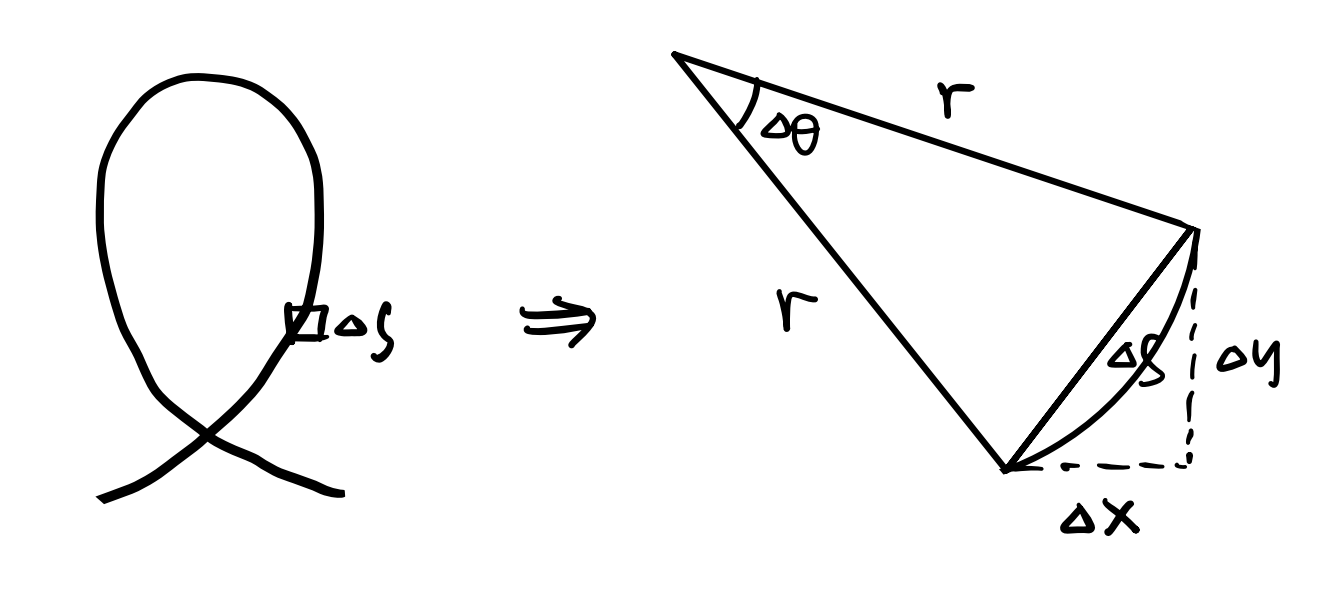
\includegraphics[width=0.3\textwidth]{1.png}
   % \end{figure}

    When entering the loop, the $G$-force suddenly acts on the passengers whose maximum value is $6G_s$.

    (In [1], the author states that the maximum $G$-force can reach 12$G_s$. It's not the condition of a perfect circle. Instead, it is possible for a curve with the curvature becomes larger in the process of from top to bottom.)














\end{document}